\section{Diskreter geometrischer Kotangens-Laplacian}

\begin{equation}
  \gls{w}\left(v_i, v_j\right) = \frac{\cot\left(\alpha\left(v_i, v_j\right)\right) + \cot\left(\beta\left(v_i, v_j\right)\right)}{2}
\end{equation}
und Grad eines Knoten ist das \emph{Voronoi-Gebiet}
\begin{equation}
  \gls{d}\left(v_i\right) = \gls{a}\left(v_i\right)
\end{equation}
also die Fläche des Voronoi-Gebietes um einen Knoten~\cite{Reuter}.

Winkel $\alpha$ und $\beta$ beschreiben die Winkel, deren Kantenenden von $v_i$ und $v_j$ aufgespannt werden.
Damit ist $\gls{L}$ symmetrisch, denn in der Rückrichtung vertauschen sich nur die Werte von $\alpha$ und $\beta$.
Da $\alpha$ und $\beta$ stets im Interval $\left(0, \pi\right)$ ist der Kotangenz eindeutig definiert.
Der Winkel befindet sich aufjedenfall in diesem Intervall!

Diese Matrix ist aber weiterhin rotationsinvariant, so dass sie eigentlich uns keinen Nutzen bringt.

$\gls{A}$ beschreibt die Lage der Knoten zu ihren benachbarten Knoten? \todo{Grafik}
Das Voronoi-Gebiet gibt an, wie viele Knoten in näherer Umgebung vorhanden sind.
Je größer das Gebiet, umso isolierter ist der Knoten.
Beinhaltet also auch eine Art Abstand (aber zu allen Knoten, nicht nur zu einem).

\subsection{Intuition}

\begin{center}
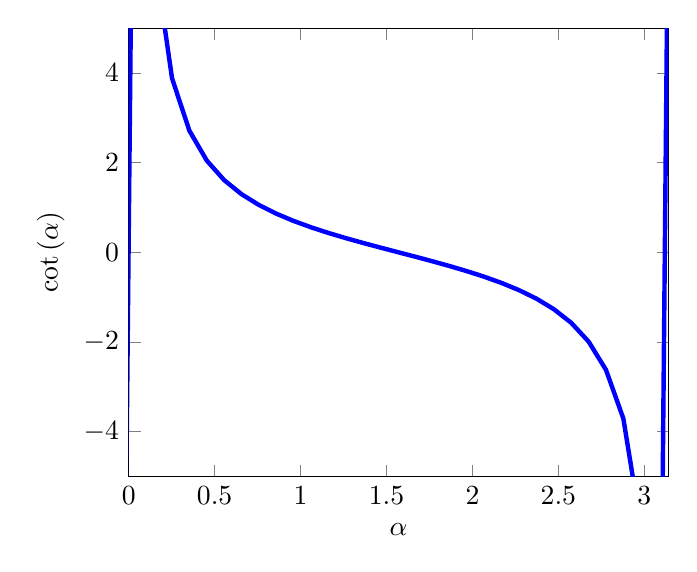
\begin{tikzpicture}
  \begin{axis}[xmax=3.14,
               xmin=0,
               ymin=-5,
               ymax=5,
               xlabel={$\alpha$},
               ylabel={$\cot\left(\alpha\right)$}]
    \addplot [samples=100, ultra thick, blue] {cos(deg(x)) / sin(deg(x))};
  \end{axis}
\end{tikzpicture}
\end{center}

Angenommen wir haben eine Kante und zwei Winkel mit $\alpha = \beta = \frac{\pi}{2}$.
Dann ist $\cot\left(\frac{\pi}{2}\right) = 0$ und wir haben $\gls{w}\left(v_i, v_j\right) = 0$.
\todo{DAS IST EXTREM KACKE}
\todo{ES GIBT AUCH NEGATIVE GEWICHTE????}

Wenn unsere Winkel sehr spitz sind, dann ist das Gewicht der Kante sehr hoch
Wenn unsere Winkel sehr stumpf sind, dann ist das Gewicht der Kante niedrig und ggf.\ negativ.

